\documentclass[11pt]{beamer}
\setbeamertemplate{navigation symbols}{}
 \setbeamercovered{transparent}
\usepackage{listings}
%\usetheme{Copenhagen}
\usetheme{Singapore}
%\usetheme{Madrid}
%\usetheme{Hannover}
%\usetheme{boxes}
%\usetheme{Boadilla}
\usefonttheme[onlymath]{serif}
\usecolortheme{beaver}
\usepackage{textpos}
\usepackage{fancyvrb}
\usepackage{xcolor}
\usepackage{multicol}
\usepackage{lipsum}
\parskip 1ex

\newcommand{\bi}{\begin{itemize}}
\newcommand{\ei}{\end{itemize}}

\newcommand\FontAcolumn{\fontsize{6}{7.2}\selectfont}
\newcommand\FontBcolumn{\fontsize{8}{7.2}\selectfont}
\newcommand\FontCcolumn{\fontsize{10}{7.2}\selectfont}
\newcommand\FontDcolumn{\fontsize{11}{7.2}\selectfont}

\definecolor{gray97}{gray}{.97}
\definecolor{gray75}{gray}{.75}
\definecolor{gray45}{gray}{.45}

\setbeamertemplate{itemize items}[square]

\lstdefinestyle{Fortran}{language=[90]Fortran}

\newcommand\FortranStyle
{
\lstset{
frame=Ltb,
framerule=0pt,
columns=fullflexible,
aboveskip=0.5cm,
framextopmargin=3pt,
framexbottommargin=3pt,
framexleftmargin=0.4cm,
framesep=0pt,
rulesep=.4pt,
backgroundcolor=\color{gray97},
rulesepcolor=\color{black},
stringstyle=\ttfamily,
showstringspaces=false,
basicstyle=\ttfamily,
commentstyle=\color{green},
keywordstyle=\color{red},
numbers=left,
numbersep=15pt,
numberstyle=\tiny,
numberfirstline=false,
breaklines=true,
 tabsize=2,
 extendedchars=true,
keepspaces,
}
}

\newcommand\FortranStyleA
{
\lstset{
frame=Ltb,
framerule=0pt,
columns=fullflexible,
aboveskip=0.5cm,
framextopmargin=3pt,
framexbottommargin=3pt,
framexleftmargin=0.4cm,
framesep=0pt,
rulesep=.4pt,
backgroundcolor=\color{gray97},
rulesepcolor=\color{black},
stringstyle=\ttfamily,
showstringspaces=false,
basicstyle=\ttfamily,
commentstyle=\color{green},
keywordstyle=\color{red},
numbersep=15pt,
numberstyle=\tiny,
numberfirstline=false,
breaklines=true,
 tabsize=2,
 extendedchars=true,
keepspaces,
}
}

\newcommand\tab[1][1cm]{\hspace*{#1}}
\newcommand{\light}[1]{\textcolor{lightgray}{#1}}
    
\def\signed #1{{\leavevmode\unskip\nobreak\hfil\penalty50\hskip2em
  \hbox{}\nobreak\hfil(#1)%
  \parfillskip=0pt \finalhyphendemerits=0 \endgraf}}

\newsavebox\mybox
\newenvironment{aquote}[1]
  {\savebox\mybox{#1}\begin{quote}}
  {\signed{\usebox\mybox}\end{quote}}


% items enclosed in square brackets are optional; explanation below
\title{Object Oriented Programming with Fortran}
\subtitle{An Overview}
\author{Carlos Cruz}
\institute{
  NASA GSFC Code 606 (ASTG)\\
  Greenbelt, Maryland 20771\\[1ex]
  \texttt{carlos.a.cruz@nasa.gov}
}
\date{October 25, 2018}



\begin{document}

% --- Title page ---
\begin{frame}[plain]
  \titlepage
\end{frame}

\logo{%
  
\includegraphics[width=1cm,height=1cm,keepaspectratio]{../../shared/nasa-ball.png}%
  \hspace{\dimexpr\paperwidth-2cm-5pt}%
  
\includegraphics[width=1cm,height=1cm,keepaspectratio]{../../shared/ssai-logo.png}%
}


% --- Slide

\begin{frame}{Agenda}

\textcolor{red}{Object Oriented Programming with Fortran}
    \bi
        \item Object Oriented Programming
        \bi
        		\item Background
        \ei
        \item OOP Features in Fortran 2003
        \bi
        	\item Data Abstraction
        	\item Encapsulation
        	\item Inheritance
        	\item Polymorphism
        \ei
        \item Examples
    \ei

\end{frame}


% --- Slide ---

\begin{frame}{Programming paradigms}
% a way of conceptualizing what it means to perform computation and how tasks to be carried out on the computer should be structured and organized
\bi
\item \textbf{Procedural}
	\bi
	\item C, Fortran90 
	\bi
		\item Focus on writing good functions and procedures %what-to-solve
		%emphasis is on doing things so that large programs are divided 
		% into smaller programs known as functions.
		\item Computation changes the program state
	\ei
	\ei
\item \textbf{Functional}
	\bi
	\item Lisp, Haskell
	\bi
		\item Emphasizes use of state-less functions %how-to-solve
	\ei
	\ei
\item \textbf{Object Oriented}
	\bi
	\item Smalltalk, Java
	\bi
		\item Programs manipulate objects
		\item Objects have an internal state
	\ei
	\ei
 \item \textbf{Multi-paradigm}
	\bi
	\item C++, Python, Fortran2003
	\ei

 \end{itemize}

\end{frame}

% --- Slide ---

\begin{frame}{Object Oriented Programming (OOP)}

OOP is a major paradigm shift. It grew out of perceived weaknesses of \emph{structured programming}:
%  SP is a programming paradigm aimed at improving the clarity, quality, and development time of a computer program by making extensive use of the structured control flow constructs of selection (if/then/else) and repetition (while and for), block structures, and subroutines.
\begin{columns}[onlytextwidth,t]
  \begin{column}{0.48\textwidth}
  \bi
   %\item Lack of support for  \textbf{encapsulation}. 
   %\bi
  \item \textcolor{magenta}{Modifications are difficult/expensive.
  \item Developers need to be expert in all parts of the application.
  \item Limited modularity.}
  %\ei
  \item [\textcolor{white}{\textbullet}] \textcolor{white}{Centralized development constraint.}

   %\item Lack of support for  \textbf{inheritance}. 
  \ei
  \end{column}
  \begin{column}{0.48\textwidth}
  \bi
  %\item Lack of support for  \textbf{polymorphism}. 
  \item [\textcolor{white}{\textbullet}] \textcolor{white}{Multiple implementations of the same functionality.}
% Support for variations leads to pervasive nested conditionals which increase complexity and errors.

  %\item Lack of support for \textbf{templates}
  \item [\textcolor{white}{\textbullet}] \textcolor{white}{Need to support several data structures that are nearly identical but vary in some systematic ways.
\item [\textcolor{white}{\textbullet}] Difficult to maintain consistency as such structures are extended.}

  \ei

  \end{column}
\end{columns}

  \vfill
  \scriptsize{
\quad \quad \quad \textcolor{magenta}{encapsulation}
\quad \quad \quad \quad \quad \quad 
\quad \quad \quad \quad \quad \quad \quad \textcolor{white}{polymorphism}\\
\quad \quad \quad \textcolor{white}{inheritance}
\quad \quad \quad \quad \quad \quad 
\quad \quad \quad \quad \quad \quad \quad \quad \textcolor{white}{templates}
}
% The main objectives of OO programming are expansibility, reusability, and compatibility.

\end{frame}

% --- Slide ---

\begin{frame}{Object Oriented Programming (OOP)}

OOP is a major paradigm shift. It grew out of perceived weaknesses of \emph{structured programming}:
%  SP is a programming paradigm aimed at improving the clarity, quality, and development time of a computer program by making extensive use of the structured control flow constructs of selection (if/then/else) and repetition (while and for), block structures, and subroutines.
\begin{columns}[onlytextwidth,t]
  \begin{column}{0.48\textwidth}
  \bi
   %\item Lack of support for  \textbf{encapsulation}. 
   %\bi
  \item \textcolor{magenta}{Modifications are difficult/expensive.
  \item Developers need to be expert in all parts of the application.
  \item Limited modularity.}
  %\ei
  \item \textcolor{cyan}{Centralized development constraint.}

   %\item Lack of support for  \textbf{inheritance}. 
  \ei
  \end{column}
  \begin{column}{0.48\textwidth}
  \bi
  %\item Lack of support for  \textbf{polymorphism}. 
  \item [\textcolor{white}{\textbullet}] \textcolor{white}{Multiple implementations of the same functionality.}
% Support for variations leads to pervasive nested conditionals which increase complexity and errors.

  %\item Lack of support for \textbf{templates}
  \item [\textcolor{white}{\textbullet}] \textcolor{white}{Need to support several data structures that are nearly identical but vary in some systematic ways.
\item [\textcolor{white}{\textbullet}] Difficult to maintain consistency as such structures are extended.}

  \ei

  \end{column}
\end{columns}

  \vfill
  \scriptsize{
\quad \quad \quad \textcolor{magenta}{encapsulation}\\
\quad \quad \quad \textcolor{cyan}{inheritance}
}
% The main objectives of OO programming are expansibility, reusability, and compatibility.

\end{frame}


\begin{frame}{Object Oriented Programming (OOP)}

OOP is a major paradigm shift. It grew out of perceived weaknesses of \emph{structured programming}:
%  SP is a programming paradigm aimed at improving the clarity, quality, and development time of a computer program by making extensive use of the structured control flow constructs of selection (if/then/else) and repetition (while and for), block structures, and subroutines.
\begin{columns}[onlytextwidth,t]
  \begin{column}{0.48\textwidth}
  \bi
   %\item Lack of support for  \textbf{encapsulation}. 
   %\bi
  \item \textcolor{magenta}{Modifications are difficult/expensive.
  \item Developers need to be expert in all parts of the application.
  \item Limited modularity.}
  %\ei
  \item \textcolor{cyan}{Centralized development constraint.}

   %\item Lack of support for  \textbf{inheritance}. 
  \ei
  \end{column}
  \begin{column}{0.48\textwidth}
  \bi
  %\item Lack of support for  \textbf{polymorphism}. 
  \item \textcolor{green}{Multiple implementations of the same functionality.}
% Support for variations leads to pervasive nested conditionals which increase complexity and errors.

  %\item Lack of support for \textbf{templates}
  \item [\textcolor{white}{\textbullet}] \textcolor{white}{Need to support several data structures that are nearly identical but vary in some systematic ways.
\item [\textcolor{white}{\textbullet}] Difficult to maintain consistency as such structures are extended.}

  \ei

  \end{column}
\end{columns}

  \vfill
  \scriptsize{
\quad \quad \quad \textcolor{magenta}{encapsulation}
\quad \quad \quad \quad \quad \quad 
\quad \quad \quad \quad \quad \quad \quad \textcolor{green}{polymorphism}\\
\quad \quad \quad \textcolor{cyan}{inheritance}
}
% The main objectives of OO programming are expansibility, reusability, and compatibility.

\end{frame}



% --- Slide ---

\begin{frame}{Object Oriented Programming (OOP)}

OOP is a major paradigm shift. It grew out of perceived weaknesses of \emph{structured programming}:
%  SP is a programming paradigm aimed at improving the clarity, quality, and development time of a computer program by making extensive use of the structured control flow constructs of selection (if/then/else) and repetition (while and for), block structures, and subroutines.
\begin{columns}[onlytextwidth,t]
  \begin{column}{0.48\textwidth}
  \bi
   %\item Lack of support for  \textbf{encapsulation}. 
   %\bi
  \item \textcolor{magenta}{Modifications are difficult/expensive.
  \item Developers need to be expert in all parts of the application.
  \item Limited modularity.}
  %\ei
  \item \textcolor{cyan}{Centralized development constraint.}

   %\item Lack of support for  \textbf{inheritance}. 
  \ei
  \end{column}
  \begin{column}{0.48\textwidth}
  \bi
  %\item Lack of support for  \textbf{polymorphism}. 
  \item \textcolor{green}{Multiple implementations of the same functionality.}
% Support for variations leads to pervasive nested conditionals which increase complexity and errors.

  %\item Lack of support for \textbf{templates}
  \item \textcolor{red}{Need to support several data structures that are nearly identical but vary in some systematic ways.
\item Difficult to maintain consistency as such structures are extended.}

  \ei

  \end{column}
\end{columns}

  \vfill
  \scriptsize{
\quad \quad \quad \textcolor{magenta}{encapsulation}
\quad \quad \quad \quad \quad \quad 
\quad \quad \quad \quad \quad \quad \quad \textcolor{green}{polymorphism}\\
\quad \quad \quad \textcolor{cyan}{inheritance}
\quad \quad \quad \quad \quad \quad 
\quad \quad \quad \quad \quad \quad \quad \quad \textcolor{red}{templates}
}
% The main objectives of OO programming are expansibility, reusability, and compatibility.

\end{frame}


% --- Slide

\begin{frame}{What is OOP?} 

OOP is a paradigm in which a program's state and behavior are bundled into \textbf{objects}.
\begin{columns}
    \begin{column}{0.48\textwidth}
        
%\begin{center} 
  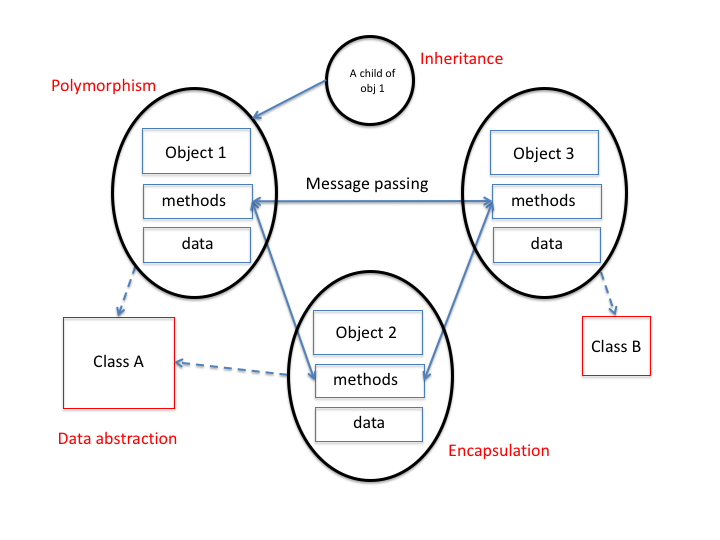
\includegraphics[width=1.2\textwidth]{../../shared/oop_features.png} 
%\end{center} 

  \end{column}
  \begin{column}{0.48\textwidth}
\scriptsize{
    \begin{itemize}
        \item A \textbf{class} is a data type
        \bi
        		\item \scriptsize{Attributes}
		\item \scriptsize{Behaviors}
        \ei
        \item An \textbf{Object} is an \textbf{instance} of a class.
        \begin{itemize}
        \item \scriptsize{Behavior of objects is expressed in terms of methods which are the class procedures. Methods have privileged access to object state.}
        \item \scriptsize{Method invocation may look different than regular procedure calls.}
        \end{itemize}
        %\item 
    \end{itemize}
 }
  \end{column}
\end{columns}
\scriptsize{Within a program, objects interact with each other by sending messages (i.e. invoking methods)}

\end{frame} 

% --- Slide

\begin{frame}{Caveats} 

    \begin{itemize}
	\item OOP is a major paradigm shift which generally takes years to fully absorb.
        \item We hope to \emph{motivate} the rationale for using OO Fortran in some circumstances.
    \end{itemize}

How do we write Fortran programs using the OO paradigm?
What OOP support does Fortran provide?

\end{frame} 


% --- Slide ---
\begin{frame}[fragile]
\frametitle{}


\centering{
\huge{
A simple example.
}
}

\end{frame}

% --- Slide

\begin{frame}{Geometrical Shapes} 
\begin{center} 
  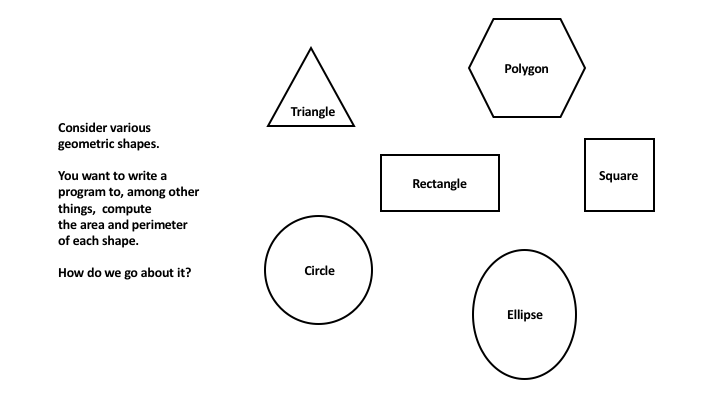
\includegraphics[width=0.9\textwidth]{../../shared/shapes0.png} 
\end{center} 

\end{frame} 


% --- Slide

\begin{frame}{Abstraction and Inheritance} 

\begin{center} 
  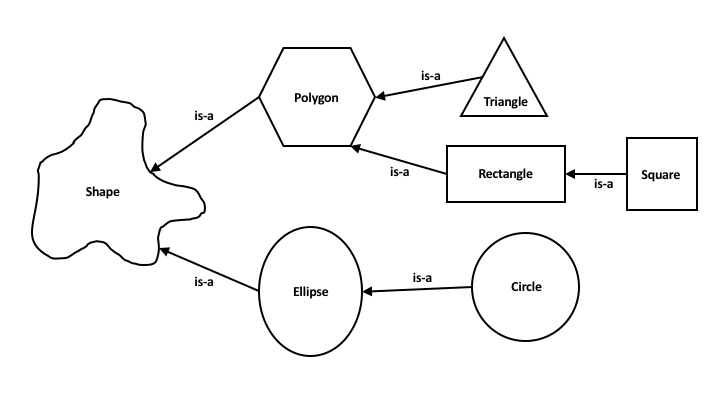
\includegraphics[width=0.9\textwidth]{../../shared/shapes.png} 
\end{center} 

\end{frame} 


% --- Slide ---

\begin{frame}[fragile]{Encapsulation (1)}
% controls visibility of names
\textbf{Encapsulation} is the ability to isolate and hide implementation details within a software subsystem.\footnote{Note: Fortran 90 introduced strong encapsulation capabilities with public/private access for module entities.}
\bi
\item Encapsulation allows the creation of an object
\item It is the mechanism can shield from outside interference or misuse. 
\bi
\item Within an object, \emph{some} of the code and/or data may be private to the object and inaccessible to anything outside the object. In Fortran we use the keyword \textbf{abstract}.
\ei
\ei

\end{frame}

% --- Slide ---

\begin{frame}[fragile]{Encapsulation (2)}

The Fortran concepts for encapsulation are \emph{derived types} and \emph{type bound procedures}\footnote{Introduced in Fortran 2003}
\footnotesize{
\FortranStyle
\begin{lstlisting}[style=Fortran]
module my_mod
   implicit none
   private ! hide everything by default
   public my_type ! expose my_type
   type my_type ! a derived type
      private ! hide data details
      real :: value
   contains
      procedure :: compute ! a public type-bound procedure
   end type my_type
end my_mod
\end{lstlisting}
}

\end{frame}


% --- Slide ---

\begin{frame}{Data Abstraction}
Abstraction can be thought of as a natural extension of encapsulation.
% In object-oriented design, programs are often extremely large. And separate objects communicate with each other a lot. So maintaining a large codebase like this for years???with changes along the way???is difficult.
% Abstraction is a concept aiming to ease this problem.
\begin{columns}

 \begin{column}{0.38\textwidth}
        
\begin{center} 
  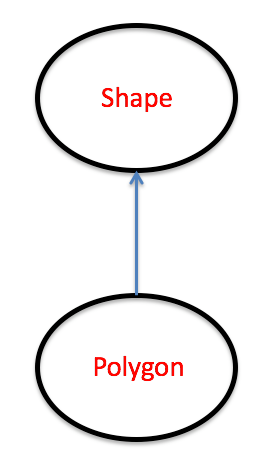
\includegraphics[width=0.7\textwidth]{../../shared/abstraction.png} 
\end{center} 

 \end{column}
  
  \begin{column}{0.7\textwidth}
%\scriptsize{
    \begin{itemize}
        \item Abstraction refers to the act of representing essential features without including the background details or explanations.
        \item Classes use concept of abstraction and are abstract data types
	\item E.g. polygon is an abstraction of shape. Shape is a generalization of polygon.
	\item Fortran 2003 supports data abstraction (keyword: \textbf{abstract})
    \end{itemize}
%	}

  \end{column}
\end{columns}
Implementation changes, e.g. a software update, rarely affect the abstraction you use.
\end{frame}

% --- Slide ---

\begin{frame}{Inheritance}
% facilitates code re-use
\textbf{Inheritance} is a way to form new classes using classes that have already been defined.
\begin{itemize}

  \item Original class is referred to as the \textbf{base} class (or \textbf{parent} class)
  \item New class is referred to as the \textbf{child} class or \textbf{subclass}
  \item Intent is to reuse significant portions of base class.
  \item Inheritance relations always form hierarchical trees.
  % Remember - the big wins are for complex software with many complex data structures.
  \item Fortran 2003 introduces inheritance (keyword: \textbf{extends})
  \item Child class should be usable in any context where the base class is usable.
  %Child class may add additional fields/components
 % Child class may override some methods of the parent class and leave other behaviors unchanged.
  \begin{itemize}
  \item Useful notion: "is-a" relationship categorization:
    \begin{itemize}
    \item frog is-a kind of amphibian
    \item sparse-matrix is-a kind of matrix
    \item polygon is-a kind of shape
    \end{itemize}
  \end{itemize}
  
 \end{itemize}

\end{frame}


% --- Slide ---

\begin{frame}{Polymorphism}

% accommodates various implementations

\textbf{Polymorphism} is the capability of treating objects of a subclass as though they were members of the parent class.
\begin{itemize}

  \item A \textbf{polymorphic variable} is one whose actual type is not known at compile time.
    \begin{itemize}
    \item Run-time environment calls the appropriate methods on depending on actual type (or \textbf{dynamic} type)
    \item Implemented with \textbf{dynamic binding} (usually function pointers)
    \end{itemize}

  \item Polymorphism and inheritance are distinct aspects but are typically applied together for maximum impact.
  \item E.g. polymorphic variable \emph{my\_shape} of \emph{class shape} will compute the compute area/perimeter according to type set at run time.
  
 \end{itemize}

\end{frame}


% --- Slide ---

\begin{frame}{Templates}

AKA \textbf{Parametric Polymorphism}.
\begin{itemize}

  \item Some languages support the ability to declare multiple similar classes simultaneously.
    \begin{itemize}
    \item Routines using the type then specify which case to use.
    \end{itemize}

  \item Fortran 2003 introduces a limited form\footnote{Parameterized derived types}.
    \begin{itemize}
    \item Derived types can be parameterized for \emph{kinds} and sizes.
    \item Cannot parameterize integers and reals simultaneously.
    \end{itemize}
  
 \end{itemize}

\end{frame}

% --- Slide

\begin{frame}{Design} 
UML diagram
\begin{center} 
  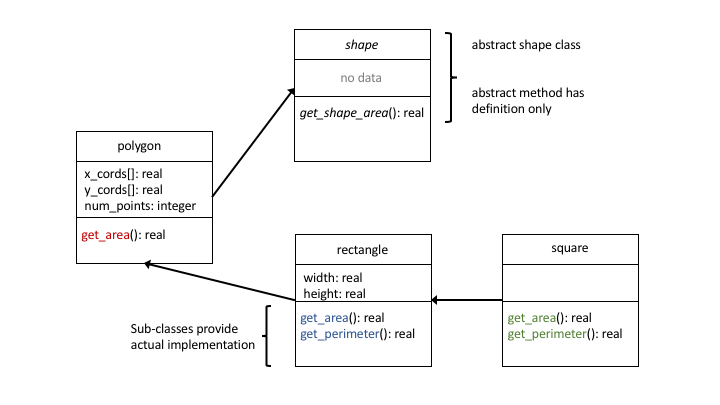
\includegraphics[width=0.9\textwidth]{../../shared/shapes_uml.png} 
\end{center} 

\end{frame} 

% --- Slide ---
\begin{frame}[fragile]
\frametitle{}


\centering{
\huge{
Complex examples.
}
}

\end{frame}

% --- Slide ---

\begin{frame}{OOP and Model Infrastructure}

The clearest case for OOP in scientific models is in the "infrastructure" which manages the various model abstractions.
\begin{itemize}

  \item Infrastructure includes
    \begin{itemize}
    \item I/O
    \item Computational grid
    \item Loop constructs
    \item Domain decomposition
    \item Calendars/clocks
    \end{itemize}

  \item Common infrastructure issues among various Earth system models led to the creation of the ESMF\footnote{Earth System Modeling Framework}. While not truly OO, ESMF is strongly encapsulated and has an object based look-and-feel.
  
 \end{itemize}

\end{frame}


% --- Slide ---

\begin{frame}{Other examples with significant use of Fortran 2003}

\begin{itemize}

  \item NASA GISS modelE tracer infrastructure 
  \begin{itemize}
  \item Supports \textbf{multiple} tracer/chemistry groups
  \item Needs to support multiple integration schemes
  \end{itemize}

  \item The parallel Fortran logging framework for HPC applications 
  \begin{itemize}
  \item Supports multiple \textbf{logging} levels and multiple \textbf{output} streams
  \end{itemize}
  
  \item pFUnit: A parallel Fortran unit testing framework for HPC applications
  
 \end{itemize}

\end{frame}

% --- Slide

\begin{frame}[fragile]
\frametitle{Conclusion}

\FontCcolumn

\begin{itemize}
\item F2003 includes a solid support of object orientation.
\item Provides opportunities to adopt newer technologies and modernize current earth science models.
\item There is already a F2008 standard, but enhancements are "minor" (submodules, co-arrays).
\end{itemize}

\bigskip
References:
\begin{itemize}
\item John Reid, "The new features of Fortran 2003, ACM SIGPLAN Fortran Forum 96", 10 (2007)
\item http://www.nag.com/nagware/NP/doc/nag\_f2003.pdf
\item http://www.pgroup.com/doc/pgifortref.pdf
\end{itemize}
\end{frame}

\end{document}